\documentclass{article}

% if you need to pass options to natbib, use, e.g.:
%     \PassOptionsToPackage{numbers, compress}{natbib}
% before loading neurips_2020

% ready for submission
% \usepackage{neurips_2020}

% to compile a preprint version, e.g., for submission to arXiv, add add the
% [preprint] option:
    %   \usepackage[preprint]{neurips_2020}

% to compile a camera-ready version, add the [final] option, e.g.:
       \usepackage[final]{neurips_2020}

% to avoid loading the natbib package, add option nonatbib:

    % \usepackage[nonatbib]{neurips_2020}


\usepackage[utf8]{inputenc} % allow utf-8 input
\usepackage[T1]{fontenc}    % use 8-bit T1 fonts
\usepackage{hyperref}       % hyperlinks
\usepackage{url}            % simple URL typesetting
\usepackage{booktabs}       % professional-quality tables
\usepackage{amsfonts}       % blackboard math symbols
\usepackage{nicefrac}       % compact symbols for 1/2, etc.
\usepackage{microtype}      % microtypography
\usepackage{authblk}
\usepackage{graphicx}
\usepackage{multirow}

\title{NNTI-2021 FINAL NLP PROJECT REPORT \newline 		HINDI/BENGALI SENTIMENT ANALYSIS}


\author{
\begin{tabular}[t]{cc} 
  Shahrukh Khan & \hspace{4cm} Mahnoor Shahid\\
  \texttt{shkh00001@uni-saarland.de} & \hspace{2cm} \texttt{mash00001@uni-saarland.de} \\
  \textbf{matriculation number 7003144} & \hspace{2cm} \textbf{matriculation number 7003144}
\end{tabular}
}


\begin{document}

\maketitle


\begin{abstract}
 This part of report is abstract. Lorem ipsum dolor sit amet, consetetur sadipscing elitr, sed diam nonumy eirmod tempor invidunt ut labore et dolore magna aliquyam erat, sed diam voluptua. At vero eos et accusam et justo duo dolores et ea rebum. Stet clita kasd gubergren, no sea takimata sanctus est Lorem ipsum dolor sit amet.
\end{abstract}


\section{Submission of NNTI Final Project 2021}

NLP task was selected. Bleh bleh bleh bleh. Below you can find the link to the project repository. 
\begin{center}
  \url{https://github.com/shahrukhx01/nnti_hindi_bengali_sentiment_analysis}
\end{center}

\section{Task One: Word Embeddings}
\label{gen_inst}

In this first task, we are provided with HASOC Hindi Sentiment Dataset and we have to create our own Word Embeddings from scratch and train a Word2Vec model which is better approach than one-hot encoding. To begin with, we have done the pre-processing of the dataset where we have removed the punctuation, usernames and stop-words[1], along with normalizing the text data to lower case. We have then obtained 20526 sorted unique words from our Hindi dataset that we have mapped with indices via 2 dictionaries: word2index (every word with an index value) and index2word (every index value with a word). We have then defined the method for one-hot-encoding as the first layer of word2vec model takes in the encoded vector and sampling probability is applied to know the probability of keeping the word in the context using the specified sub-sampling formula which is used by get\_target\_context method to generate what skip gram model requires. Afterwards, we have developed the Word2Vec model and trained the dataset onto this to get the desired Word Embeddings.

\section{Influence of Hashtags and Emojis on Sentiment Analysis of the Hindi Dataset}
\label{headings}

In general, the usage of hashtags in a sentence can benefit us in investigation under many various aspects, one of the common ones that includes Context Identification, Sentiment Analyses etc. Mostly, there is great influence of hashtags on the sentences:

\begin{itemize}
    \item As just by observing the words that are used as hashtags or by perceiving the high volumes of certain hashtags can direct us to the subject of the content or the trending topic. 
   \item Correspondingly, it can affect the strength of the sentiment in a sentence, for example multiple negative hashtags can increase the negative sentiment of a tweet.
\end{itemize}

For these certain reasons we have settled not to eliminate them. 

Our dataset is consisting of tweets in the targeted languages; Hindi and Bengali, and these text sentences are provided to us, marked already with the flags: HOF and NOT [2] as shown in Table 1 so we will be using these indicators to segregate whether the hashtags belong to a negative sentence or non-negative sentence, to know how much proportion of hate speech our dataset has.

\begin{table}

  \caption{Flags marked on Hindi Dataset and their meanings}
  \label{Table 3.0}
  \centering
  \begin{tabular}{cl}
    \toprule                \
    Flag     & What it means \\
    \midrule
    HOF (Hate and Offensive)     & Tweets that contains hate, offensive and aggressive words are \\ & labeled using this \\
    NOT (Non Hate-Offensive)     & Tweets that has no indication of any hate and offensive words are \\ & labeled using this.  \\
    \bottomrule
  \end{tabular}
\end{table}


\subsection{Dividing the tweets into negative vs non-negative sentences}

Before we have extracted the hashtags from the dataset, we have divided the data based on the flags \textbf{HOF} and \textbf{NOT}, so that we can get to know the proportion of negative and non-negative text sentences in our provided Hindi Dataset. As shown in Table 1, we can perceive that our dataset has almost equal ratio of negative and non-negative sentences. 

\begin{table}[b]
\begin{center}
  \caption{Tweets divided into Negative vs NonNegative Sentences}
  \centering
  \begin{tabular}{p{2cm}  l p{2cm} }
    \toprule                \
    Flag     & No. of Sentences     & Proportion \\
    \midrule
    HOF     & 2469   & 52.92\% \\
    NOT     & 2196   & 47.07\%  \\
    \bottomrule
  \end{tabular}
\end{center}
\end{table}


\subsection{Extracting the hashtags from Hindi Dataset}
Once we have separated the data frames, we will extract the hashtags out of our dataset for further investigation. We have then used the matcher class from the spacy package (python library) to match the sequences of the tokens, based on pattern rules and obtained the hash tags for both the negative and non-negative sentences.

\subsection{Examining the proportion of hashtags}

For better understanding of the proportion of the hashtags that we have obtained from our Hindi dataset, we will visualize the tags in the pie chart. As can be distinguished in the Figure 1, there is a remarkable difference between the hashtags we have for negative sentences in the comparison to the non-negative. We only have a total of \textbf{25.4\%}  of the hashtags from the negative sentences in our entire Hindi dataset.

\begin{figure}
  \centering
  
  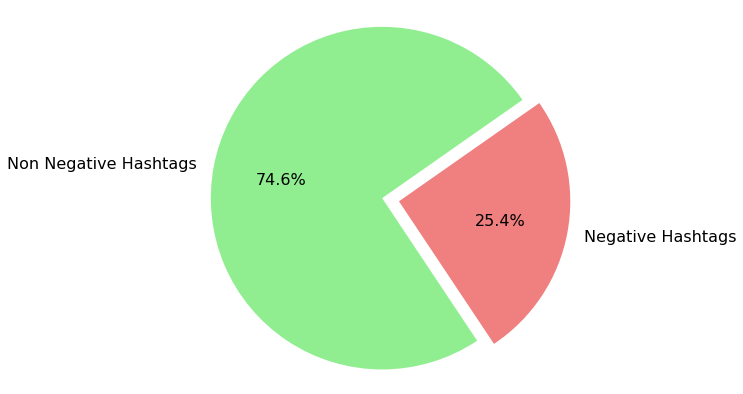
\includegraphics[width=10.2cm, height=5.5cm]{piechart.png}
%   \fbox{\rule[-.5cm]{0cm}{4cm} \rule[-.5cm]{4cm}{0cm}}
  \caption{Hastags in Hindi Dataset for Negative vs Non-Negative Sentences}
\end{figure}

\subsection{Investigating the sentiment of hashtags}

In order to extract the sentiment of the words used for hashtags, we have used TextBlob module imported from textblob (python library), since we can observe that all the hashtags in the Hindi Dataset are english alphabetic words. \textit{Subsequently, we have found 0 polarity for all the hash tags, meaning they do not provide any assistance or they have no impact in the positive and negative sentiment of sentence.} However, the frequency of a particular hashtag or the frequency of related hashtags can led us to know about the topic of the tweets. So we will further look into the frequency count.

\subsection{Detecting the content of the hashtags}

If the purpose of the study is based on the context of subject, then these hashtags in the Hindi Dataset tells us much more about that. Figure 2 is an example wordcloud that represents the most used words as the hashtags in the Hindi Dataset, where blue hashtags represent the ones used in negative sentences and the grey hashtags represent the ones used in positive sentences, interestingly, from which we can spot that even though the proportion of the Negative Hashtags was one-fourth in contrast to Non-Negative hashtags, the most frequent hashtags were the negative ones and the topics on which we will have the hate-speech are the tweets mostly regarding politics and cricket matches.

\begin{figure}[b]
  \centering
  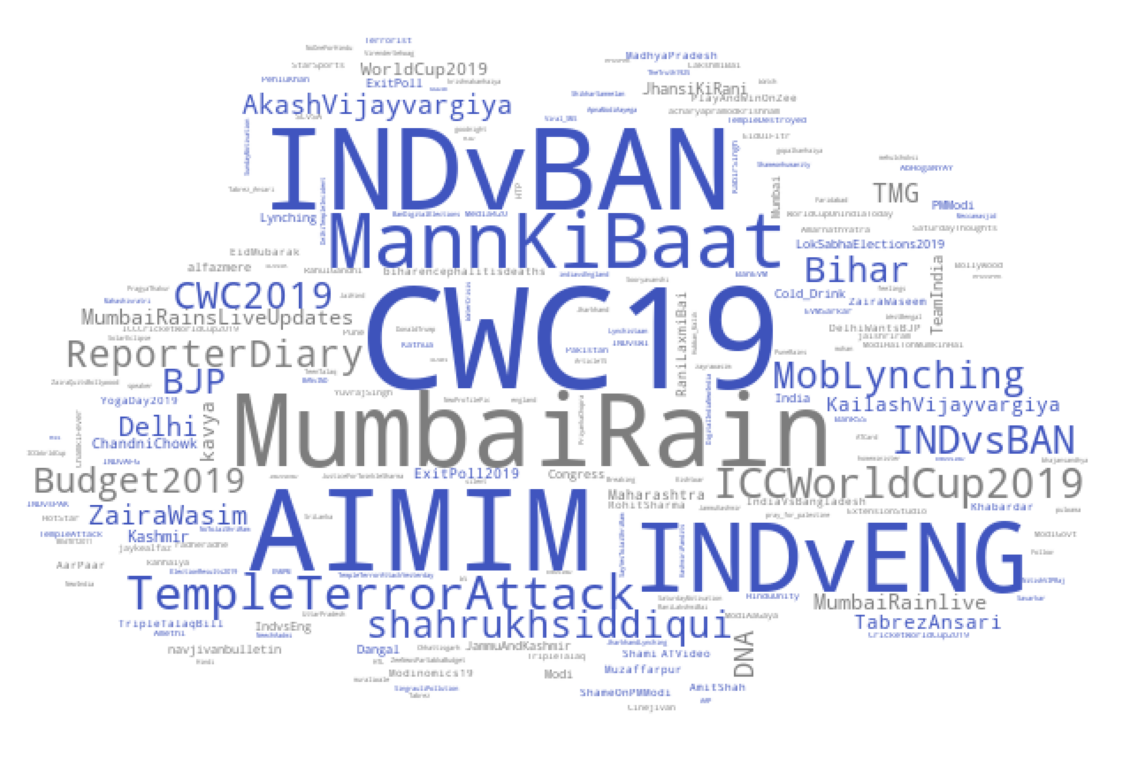
\includegraphics[width=12cm, height=6cm]{wordcloud2.png}
%   \fbox{\rule[-.5cm]{0cm}{4cm} \rule[-.5cm]{4cm}{0cm}}
  \caption{WordCloud indicating the most frequent hashtags in the Hindi Dataset}
\end{figure}

\subsection{Further exploration for the emojis}
Emoticons, also referred as emojis are unicode graphical symbols, which are used to articulate and convey the sentiment in a sentence. By analyzing the sentiment of the emojis we can draw several noteworthy conclusions which might be motivating to the study of interest. 
Hence, with the intention to obtain the emojis from the Hindi Dataset we have used regex and have specified all the Emoji Unicode Blocks in the pattern and have used the findall() method to get the list of emojis, regrettably we have just 2 emojis in the entire dataset. \textit{So, removing them and not removing them will not make any difference in this setting.  }

\section{Hyperparameters for the Word2Vec Model created in Task One}
\label{others}

By setting different values for hyperparameters with different combinations, this was observed that for the better performance of the model, they should be set to Epochs = 500, Window Size = 2, Embedded Size = 300, and Learning Rate = 0.05, in our case of study.


\subsection{Examining the different values of window size for the model with embedded size = 300}

Successively, executing the model using the combinations of values for the hyperparameters, as described in Table 3, the loss rate was considerably low for window size = 1 and window size = 2 and was increasing with the raise in the number of window size. Moreover, the loss rate shoots up abruptly for higher window size values when executed for more epochs. It is also evident from Figure 3 that loss for window size 2 converges faster as compare to window size 1. 

\begin{figure}
  \centering
  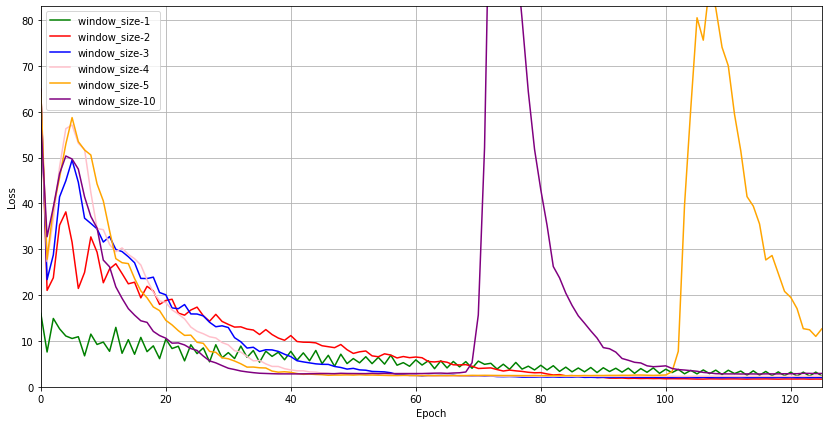
\includegraphics[width=13cm, height=6.7cm]{model_loss_window_sizes.png}
%   \fbox{\rule[-.5cm]{0cm}{4cm} \rule[-.5cm]{4cm}{0cm}}
  \caption{Loss of model for different values of window size with fixed embedded size = 300}
\end{figure}

\subsection{Examining the different values of learning rate for the model with embedded size = 300 and window size = 2}

From table 3, we can note that by decreasing the learning rate to 0.01 or increasing the learning rate to 0.1 did not provide us any significantly better result.

\begin{table}[b]
\begin{center}
  \caption{Different combinations of hyper parameters}
  \centering
  \begin{tabular}{c|ccc}
    \toprule    
    
    Embedded Size & Learning Rate  & Window Size  & Min Loss Score\\
    \midrule
    \multirow{9}{*}{300} & \multirow{6}{*}{0.05} & 1 & 0.841\\
    & & 2  & 1.559  \\
    & &3 & 1.942 \\
    & &4 & 2.151\\
    & &5  & 2.321\\
    & &10 & 2.792\\
    \cmidrule(r){2-4}
    & \multirow{3}{*}{0.01} & 1 & 1.298 \\
    & & 2 & 3.295 \\
    & & 10 & 2.747 \\
    \cmidrule(r){2-4}
    & \multirow{3}{*}{0.1} & 1 & 1.311 \\
    & & 2 & 1.557 \\
    & & 10 & 3.551 \\

    \bottomrule
  \end{tabular}
\end{center}
\end{table}

\section{Setting the Optimizer and Loss Function for the model in Task One}

Lorem ipsum dolor sit amet, consetetur sadipscing elitr, sed diam nonumy eirmod tempor invidunt ut labore et dolore magna aliquyam erat, sed diam voluptua. At vero eos et accusam et justo duo dolores et ea rebum. Stet clita kasd gubergren, no sea takimata sanctus est Lorem ipsum dolor sit amet.

\section{Task Two: Sentiment Classifier \& Transfer Learning}

Lorem ipsum dolor sit amet, consetetur sadipscing elitr, sed diam nonumy eirmod tempor invidunt ut labore et dolore magna aliquyam erat, sed diam voluptua. At vero eos et accusam et justo duo dolores et ea rebum. Stet clita kasd gubergren, no sea takimata sanctus est Lorem ipsum dolor sit amet.



\section{Results}

Lorem ipsum dolor sit amet, consetetur sadipscing elitr, sed diam nonumy eirmod tempor invidunt ut labore et dolore magna aliquyam erat, sed diam voluptua. At vero eos et accusam et justo duo dolores et ea rebum. Stet clita kasd gubergren, no sea takimata sanctus est Lorem ipsum dolor sit amet.

\section{Conclusion}

Lorem ipsum dolor sit amet, consetetur sadipscing elitr, sed diam nonumy eirmod tempor invidunt ut labore et dolore magna aliquyam erat, sed diam voluptua. At vero eos et accusam et justo duo dolores et ea rebum. Stet clita kasd gubergren, no sea takimata sanctus est Lorem ipsum dolor sit amet.

\section*{References}

References follow the acknowledgments. Use unnumbered first-level heading for
the references. Any choice of citation style is acceptable as long as you are
consistent. It is permissible to reduce the font size to \verb+small+ (9 point)
when listing the references.
{\bf Note that the Reference section does not count towards the eight pages of content that are allowed.}
\medskip

\small

[1] Hindi Stopwords - https://github.com/stopwords-iso/stopwords-hi/blob/master/stopwords-hi.txt

[2] Thomas Mandl, Sandip Modha, Prasenjit Majumder, Daksh Patel, Mohana Dave, Chintak Mandlia, and Aditya Patel. Overview of the hasoc track at fire 2019: Hate speech and offensive content identification in indo-european languages. In Proceedings of the 11th Forum for Information Retrieval Evaluation, pages 14–17, 2019.


\end{document}